% !TEX program = xelatex
\documentclass[a4paper]{ctexart}
\usepackage[top=3cm, bottom=2cm]{geometry}
\usepackage{graphicx}
\graphicspath{{fig/}}
\usepackage{subcaption}
\usepackage{amsmath}
\usepackage{amssymb}
\usepackage{xcolor}
\usepackage{url}
\usepackage{booktabs}
\usepackage{multirow}
%\usepackage{hyperref}
\usepackage[hidelinks]{hyperref} % 加载 hyperref 并隐藏链接边框

%\usepackage[utf8]{inputenc}
%\usepackage[ngerman]{babel} % 加载德语支持

% booktabs 提供 \toprule, \midrule, \bottomrule 等表格命令
% (booktabs 已在第9行加载，此处不再重复)

% 定义占位命令以避免未定义控制序列错误
%\newcommand{\placeholderspace}{}
\usepackage{fancyhdr} % 导入fancyhdr宏包
\usepackage{lipsum}   % 仅用于生成示例文本

\usepackage{float}    % 提供 H 浮动位置选项
% 定义可选图像命令，避免未定义控制序列错误
\newcommand{\optionalfigure}[3]{%
    \IfFileExists{fig/#1}{%
        \begin{figure}[H]
            \centering
            \includegraphics[width=#2\textwidth]{fig/#1}
            \caption{#3}
        \end{figure}
    }{%
        \IfFileExists{#1}{%
            \begin{figure}[H]
                \centering
                \includegraphics[width=#2\textwidth]{#1}
                \caption{#3}
            \end{figure}
        }{}%
    }%
}
% 设置页面样式为fancy
\pagestyle{fancy}
% 自定义页眉内容
\fancyhead[L]{} % 左侧页眉
\fancyhead[C]{\textbf{Physics-experiment Reporting Letter:\\Spatial Light Modulator}} % 中间页眉
\fancyhead[R]{} % 右侧页眉
% 自定义页脚内容
\fancyfoot[L]{} % 左侧页脚
\fancyfoot[C]{\thepage} % 中间页脚显示页码
\fancyfoot[R]{} % 右侧页脚
% 改变页眉线的粗细
\renewcommand{\headrulewidth}{1.4pt}
% 改变页脚线的粗细
\renewcommand{\footrulewidth}{0pt}
\setlength{\headheight}{24pt}




\title{空间光调制器原理与应用}
\author{实验人：学生\qquad 学号：[学号已脱敏]\qquad 指导教师：王海波}
\date{实验日期：2026.6.5}

\begin{document}

\maketitle

\begin{abstract}
本实验研究了电寻址液晶空间光调制器（LCSLM）的基本工作原理及其在光学信息处理中的应用。实验首先利用 He-Ne 激光器、起偏器、半波片、LCSLM、检偏器和功率计组成偏振测量光路，测量灰度为 0 与 255 时透过光功率随半波片光轴角度的变化，并进一步获得输出光功率随输入灰度变化的振幅调制曲线。实验结果表明，LCSLM 对不同灰度写入信号具有明显的振幅调制作用，灰度 0 与 255 对应的角度响应曲线近似互补；在本组数据中，对比度 $I_{255}/I_0$ 的最大值约为 85.5，对应半波片角度约为 $230^\circ$。灰度--功率响应呈非线性增长，二次拟合的决定系数约为 0.9901。实验还结合 $4f$ 系统、空间滤波和计算全息再现，对黑栅效应、正负像转换及边缘像形成机理进行了定性分析。\\

\textbf{关键词：空间光调制器\quad 液晶电光效应\quad 振幅调制\quad 4f系统\quad 数字全息}
\end{abstract}

\section{引言}

空间光调制器（Spatial Light Modulator, SLM）是一类能够在空间上调制光场振幅、相位、偏振态或强度分布的器件。它通常由大量可独立控制的像素单元构成，能够把电信号或光信号所携带的信息加载到一维或二维光场中，从而充分利用光学系统高速、并行和互连的特点。

液晶空间光调制器是目前应用较广的一类 SLM。电寻址液晶空间光调制器（LCSLM）以液晶层作为调制介质，通过改变像素上的驱动电压控制液晶分子的取向，进而改变通过液晶盒的光波偏振态和相位延迟。若在 LCSLM 前后配合偏振片使用，就可以把偏振态变化转化为输出光强变化，实现振幅调制。

SLM 在光学信息处理、图像转换、空间滤波、全息显示和自适应光学等领域具有重要应用。与传统全息干版相比，LCSLM 可由计算机实时加载图像或全息图，能够快速改变调制图样，因而特别适合用于计算全息和动态光学实验。本实验通过测量 LCSLM 的振幅调制曲线，并观察图像转换、黑栅效应消除和全息图再现现象，加深对液晶空间光调制器工作机理及应用方式的理解。

\section{原理}

\subsection{液晶的电光效应}

液晶是一种介于固体与液体之间的物质相态，既具有一定的分子取向有序性，又具有流动性。常用于空间光调制器的向列相液晶分子近似为细长棒状，其折射率、介电常数等物理量在分子长轴方向与垂直方向上不同，因此表现出明显的各向异性。

当液晶盒中液晶分子取向发生变化时，入射光在液晶中经历的有效折射率也随之改变。对于非寻常光和寻常光，其折射率分别记为 $n_e$ 与 $n_o$，双折射率为
\begin{equation}
    \Delta n=n_e-n_o .
\end{equation}
液晶盒厚度为 $d$ 时，两偏振分量之间的相位延迟可写为
\begin{equation}
    \delta=\frac{2\pi}{\lambda}\Delta n d ,
\end{equation}
其中 $\lambda$ 为入射光波长。外加电场改变液晶分子的排列方向，从而改变 $\Delta n$ 与相位延迟 $\delta$，这就是液晶电控双折射效应。

\subsection{扭曲向列效应与混合场效应}

若液晶盒上下两基片的取向方向不同，液晶分子在厚度方向上会逐渐扭转，形成扭曲向列结构。对于扭曲角约为 $90^\circ$ 的液晶盒，线偏振光通过液晶层时，其偏振方向可随液晶分子取向逐渐旋转。因此在无外加电场时，若起偏器与检偏器正交，入射光仍可能由于偏振方向旋转而透过检偏器，形成亮场。

当施加电场时，正性液晶分子长轴趋向沿电场方向排列，原有的连续扭曲结构被削弱甚至破坏，出射光偏振态随之改变。液晶空间光调制器的实际调制通常同时包含扭曲向列效应和电控双折射效应，称为混合场效应。不同灰度对应不同像素驱动电压，因此可产生不同的偏振态和透过光强。

\subsection{电寻址 LCSLM 与振幅调制}

电寻址 LCSLM 由二维像素阵列构成。每个像素对应一个可独立控制的透明电极，计算机输出图像的灰度值通过驱动电路转化为相应电压，控制对应区域液晶分子的取向。照明整个器件的光称为读出光，被调制后的光称为输出光。

在振幅调制实验中，读出光先经过起偏器成为线偏振光，再通过半波片调节偏振方向与液晶取向之间的夹角。LCSLM 改变出射光的偏振态，检偏器则把这种偏振态变化转化为光强变化。若以灰度 $g$ 表示写入信号，输出光功率可记为
\begin{equation}
    P=P(g,\theta),
\end{equation}
其中 $\theta$ 为半波片光轴角度。通过测量不同 $\theta$ 和不同灰度下的 $P$，即可得到 LCSLM 的振幅调制特性。

\subsection{黑栅效应与 4f 系统}

实际 LCSLM 的像素之间存在不透明的控制电路区域，通常称为黑栅。黑栅一方面降低有效开口率和光利用效率，另一方面相当于二维周期光栅，会使输出光产生阵列状衍射斑，从而影响成像质量。

消除黑栅效应的一种常见方法是采用 4f 空间滤波系统。两个焦距相同的傅里叶透镜 $L_1$、$L_2$ 同轴共焦放置，输入面位于 $L_1$ 的前焦面，频谱面位于两透镜公共焦面，输出面位于 $L_2$ 的后焦面。若在频谱面放置光阑，挡去由黑栅引起的高阶衍射频谱，仅保留主要低频信息，就可以减弱黑栅结构对成像的影响。

\subsection{数字全息图再现}

计算全息通过计算机将目标光场的复振幅分布转化为可加载的全息图。其基本过程包括：对目标波前进行离散采样，利用快速傅里叶变换计算频谱，进行编码并生成适合 LCSLM 显示的灰度图，再用相干光照明 LCSLM 实现光学再现。

在振幅型 LCSLM 上加载计算全息图后，透过检偏器的输出光包含目标图像的频谱信息。经过傅里叶透镜后，在焦平面附近可以观察到再现图像。由于振幅型器件无法独立调制完整复振幅，实际再现结果常伴随零级光、共轭像和背景噪声，需要通过光路调节和空间滤波改善。

\section{实验}

\subsection{实验装置}

本实验光路主要由 He-Ne 激光器、起偏器、半波片、LCSLM、检偏器、功率计、扩束准直系统、傅里叶透镜、光阑和 CMOS 摄像头等部分构成。He-Ne 激光器输出波长为 $632.8\,\mathrm{nm}$ 的相干光；起偏器用于获得线偏振读出光；半波片用于连续调节入射偏振方向；LCSLM 接收计算机输出的灰度图像并调制读出光；检偏器和功率计用于测量振幅调制特性；扩束准直系统与 4f 系统用于图像转换、空间滤波和全息再现观察。

\optionalfigure{setup.jpg}{0.82}{空间光调制器实验光路照片}

\subsection{实验步骤}

实验首先搭建偏振测量光路，调节激光、起偏器、半波片、LCSLM 和检偏器，使功率计能够稳定接收透过光。将 LCSLM 输入图像分别设为灰度 0 和灰度 255，改变半波片光轴角度，记录透过光功率随角度的变化。由同一角度下两灰度对应功率的比值计算对比度，并寻找对比度较大的工作角度。

随后固定半波片在选定工作状态附近，以 25 为步长改变输入图像灰度，测量输出光功率，得到 LCSLM 的灰度--功率响应曲线。该曲线反映输入灰度、液晶驱动电压和输出光强之间的综合关系，是评价振幅型 SLM 工作特性的重要依据。

在图像转换与黑栅效应实验中，在基础光路上加入扩束镜和准直镜，使入射到 LCSLM 的光近似为平行光，并将 LCSLM、两个傅里叶透镜和 CMOS 摄像头按 4f 系统摆放。通过在频谱面放置或移除光阑，比较成像结果中黑栅衍射结构的变化。旋转半波片时，观察正像、负像以及边缘增强、边缘减弱等图像。

在数字全息再现实验中，将计算得到的全息图加载到 LCSLM 上，调节 CMOS 位置至合适观察面，记录再现图像。若进行像素尺寸测量，可把 LCSLM 视作二维透射光栅，通过夫琅和费衍射斑间距反推出像素周期。

\section{结果与分析讨论}

\subsection{灰度 0 与 255 的功率--角度关系}

由实验数据绘制灰度 0 与灰度 255 时透过光功率随半波片光轴角度变化的曲线，如图 \ref{fig:power-angle} 所示。

\begin{figure}[H]
    \centering
    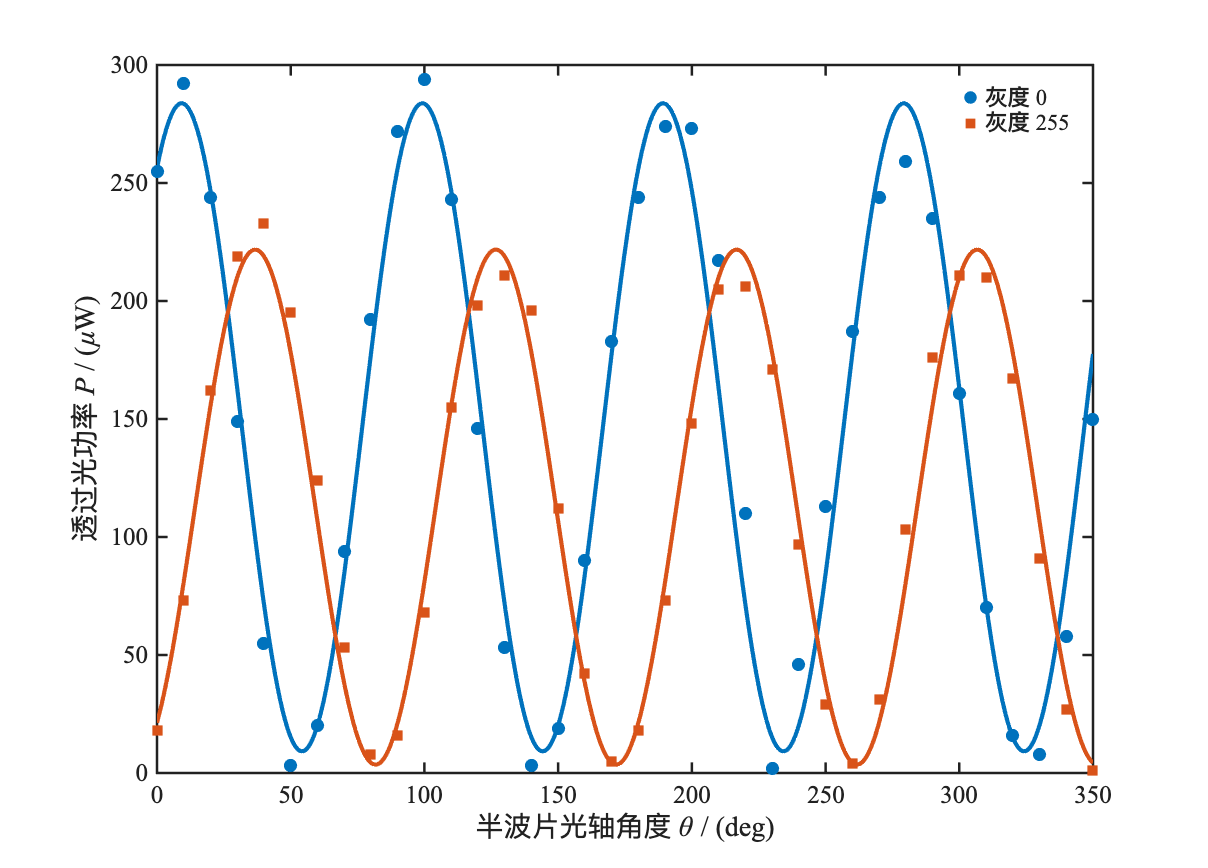
\includegraphics[width=\textwidth]{power_angle.png}
    \caption{灰度 0 与 255 时透过光功率随半波片角度的变化}
    \label{fig:power-angle}
\end{figure}

可以看出，两条曲线均随半波片角度呈周期性变化，这是因为半波片改变了入射线偏振光相对于液晶取向和检偏器透光轴的方向。灰度 0 与灰度 255 两种状态下的曲线近似互补：当灰度 0 对应输出较强时，灰度 255 往往对应较弱输出，反之亦然。这说明 LCSLM 的写入灰度确实改变了液晶盒对偏振光的调制状态，使检偏器后的透过光强发生显著变化。

由于实际液晶盒并非理想相位延迟器，且光路中存在偏振片消光比有限、LCSLM 像素不均匀、光束准直误差等因素，两条曲线并不完全呈严格的正弦互补关系。尤其在局部极小值附近，微小背景光、散射光和仪器零点误差都会使功率比值出现较大波动。

\subsection{对比度与最佳工作角度}

根据数据表中定义，对比度取为同一半波片角度下灰度 255 与灰度 0 的透过功率比值：
\begin{equation}
    C(\theta)=\frac{I_{255}(\theta)}{I_0(\theta)} .
\end{equation}
计算得到的对比度曲线如图 \ref{fig:contrast-angle} 所示。

\begin{figure}[H]
    \centering
    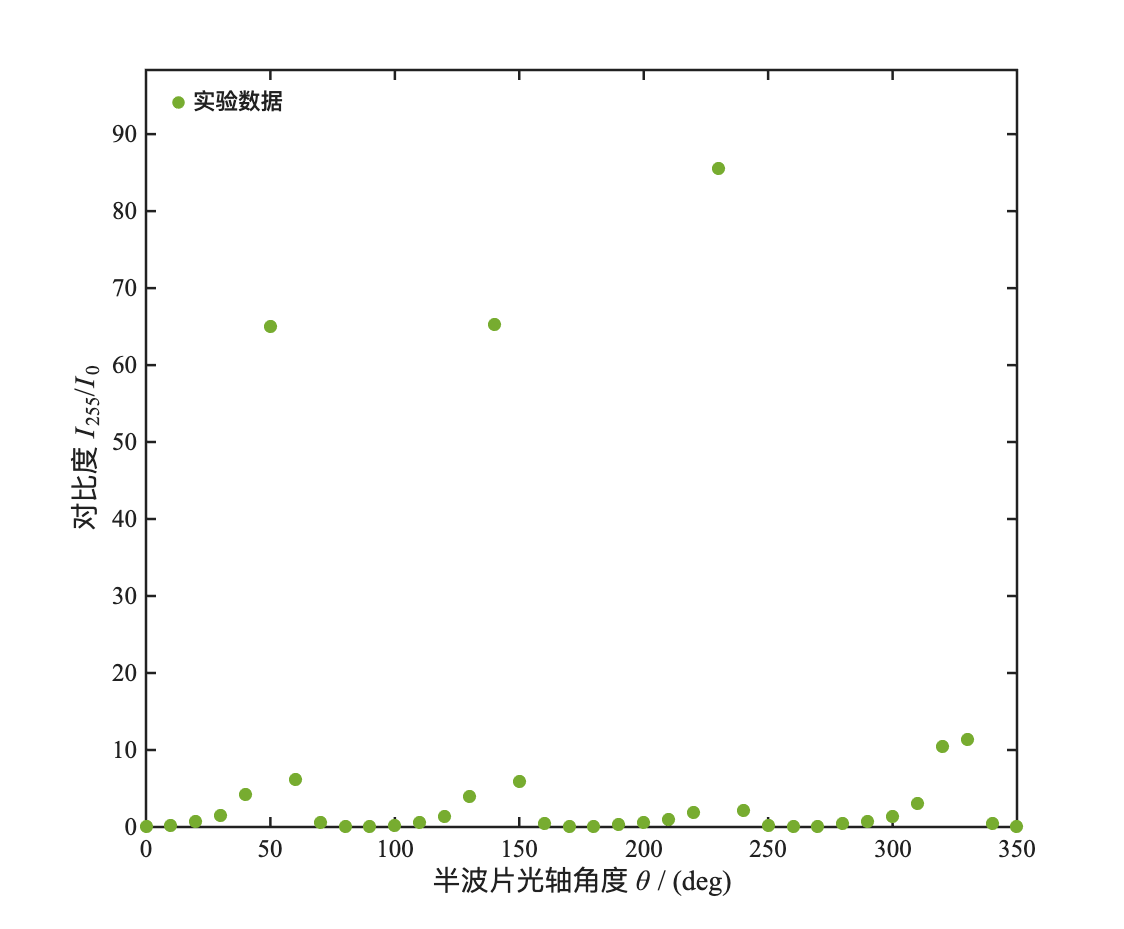
\includegraphics[width=0.88\textwidth]{contrast_angle.png}
    \caption{对比度 $I_{255}/I_0$ 随半波片角度的变化}
    \label{fig:contrast-angle}
\end{figure}

本组数据中，对比度最大值出现在 $\theta=230^\circ$ 附近，此时灰度 0 的透过功率约为 $2\,\mu\mathrm{W}$，灰度 255 的透过功率约为 $171\,\mu\mathrm{W}$，对应
\begin{equation}
    C_{\max}=\frac{171}{2}=85.5 .
\end{equation}
该角度可作为振幅调制实验中较适合的工作角度，因为两种极端灰度对应的输出光强差异最明显。

需要注意的是，最大对比度出现在灰度 0 输出功率接近极小值的位置，因此该数值对暗电流、背景光和功率计读数误差较为敏感。若以实际成像质量为目标，工作角度不仅要追求高对比度，还应兼顾整体透过率和图像亮度。

\subsection{灰度--功率响应曲线}

在选定偏振工作状态下，改变 LCSLM 输入图像灰度并记录输出光功率，得到灰度--功率响应曲线，如图 \ref{fig:gray-response} 所示。

\begin{figure}[H]
    \centering
    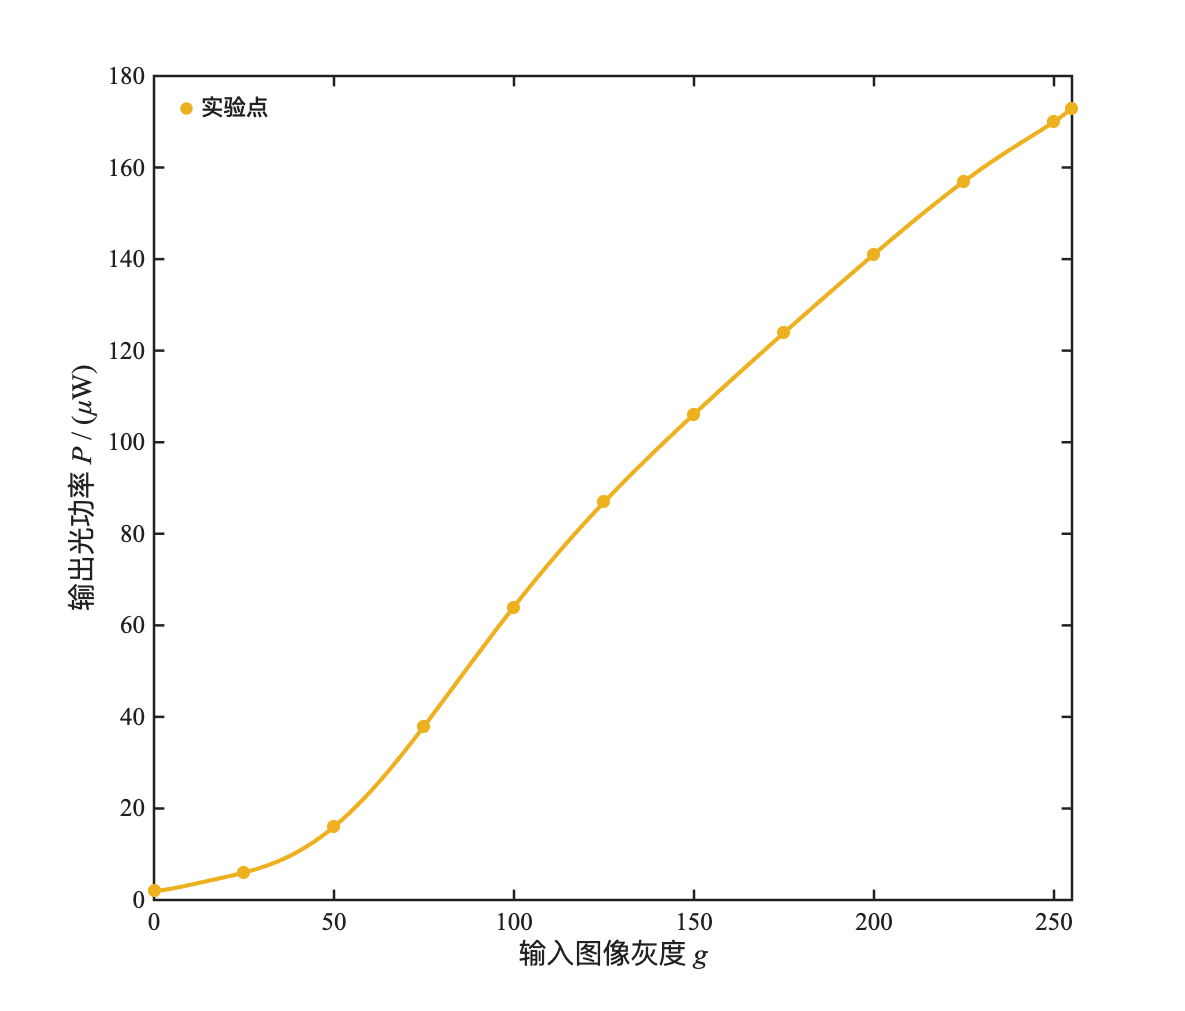
\includegraphics[width=0.88\textwidth]{gray_response.png}
    \caption{LCSLM 输出光功率随输入灰度的变化}
    \label{fig:gray-response}
\end{figure}

实验数据表明，输出功率随灰度增大而单调上升，但并非严格线性关系。

曲线的非线性来源于多个因素：首先，灰度值与实际加载在液晶像素上的电压之间可能不是线性关系；其次，液晶分子取向随电压变化本身存在阈值效应和饱和趋势；最后，检偏器后的光强还与偏振态变化之间满足类似马吕斯定律的非线性关系。因此，在需要精确灰度控制的应用中，应先测量并标定振幅调制曲线，再根据目标光强反求所需灰度。

\subsection{图像转换与黑栅效应}

在图像转换实验中，LCSLM 加载灰度图像后，每个像素对入射光进行局域振幅调制，因而输出光场携带了输入图像信息。通过 4f 系统可以在输出面观察到对应图像。旋转半波片会改变 LCSLM 振幅调制曲线的工作点，使同一输入灰度对应的输出透过率发生反转或重新分配，因此可观察到正像和负像的转换。

\optionalfigure{zheng.png}{0.65}{LCSLM 图像转换实验中观察到的正像}
\optionalfigure{fu.png}{0.65}{LCSLM 图像转换实验中观察到的负像}

边缘增强与边缘减弱可以从空间频率角度理解。图像边缘对应较高空间频率分量，若 4f 系统频谱面上的光阑选择性改变不同空间频率的通过情况，就会改变边缘与低频背景之间的相对强度。当高频成分相对增强时，边界轮廓更清楚，表现为边缘增强；当高频成分被抑制时，图像边缘变得模糊，表现为边缘减弱。

\optionalfigure{bianyuan.png}{0.65}{4f 系统空间滤波得到的边缘像}

LCSLM 像素间黑栅具有周期结构，会在频谱面形成规则的高阶衍射点。这些衍射分量若进入第二个傅里叶透镜，就会在像面引入周期性条纹或多重像，降低成像质量。在频谱面加入光阑后，高阶衍射分量被部分挡去，因此黑栅结构造成的干扰减弱，图像背景更干净。不过光阑过小时也会损失图像高频信息，使细节变模糊。

\optionalfigure{filter_compare.jpg}{0.82}{4f 系统频谱面有无光阑时的成像效果对比}

\subsection{数字全息再现与像素尺寸测量}

数字全息再现实验中，计算机生成的全息图被加载到 LCSLM 上，LCSLM 作为可更新的全息载体调制入射相干光。经透镜进行傅里叶变换后，可在合适观察面看到再现图像。由于本实验采用振幅型调制，并且系统中存在零级光、黑栅衍射以及 LCSLM 有限像素尺寸等影响，再现图像通常伴随背景亮斑和衍射噪声。通过调整检偏器角度、改变全息图显示位置、遮挡零级光或进行空间滤波，可以提高再现图像的可辨识度。

\optionalfigure{hologram_reconstruction.jpg}{0.65}{LCSLM 加载计算全息图后的再现图像及衍射斑间距测量}

图中可以看到中心零级亮斑附近存在近似矩形排列的红色衍射点阵，这是 LCSLM 像素周期结构对相干光产生的二维光栅衍射。照片中同时放置了毫米刻度尺，因此可由图像估读衍射斑间距。以尺上 $1\,\mathrm{cm}$ 刻度对应的图像长度作为标定，得到
\begin{equation}
    1\,\mathrm{cm}\approx 117\,\mathrm{pixel}.
\end{equation}
对图中多组清晰的相邻衍射点进行读数，得到相邻级间距约为
\begin{equation}
    \Delta N=(40.8\pm1.9)\,\mathrm{pixel},
\end{equation}
因此屏上零级与一级衍射斑间距为
\begin{equation}
    x=\frac{\Delta N}{117}\,\mathrm{cm}
      \approx (0.349\pm0.016)\,\mathrm{cm}
      =(3.49\pm0.16)\,\mathrm{mm}.
\end{equation}

利用夫琅和费衍射测量 SLM 像素大小时，可将 LCSLM 的像素阵列视为二维光栅。设像素周期为 $d$，入射波长为 $\lambda$，第 $m$ 级衍射角为 $\theta_m$，则满足
\begin{equation}
    d\sin\theta_m=m\lambda .
\end{equation}
若在焦距为 $f$ 的透镜焦平面上测得零级与一级衍射斑间距为 $x$，小角近似下有
\begin{equation}
    \sin\theta_1 \approx \tan\theta_1 \approx \frac{x}{f},
\end{equation}
因此像素周期可由
\begin{equation}
    d \approx \frac{\lambda f}{x}
\end{equation}
求得。本实验采用 He-Ne 激光，$\lambda=632.8\,\mathrm{nm}$。代入照片读得的 $x$，若 $f$ 以 $\mathrm{mm}$ 为单位，则
\begin{equation}
    d(\mu\mathrm{m})\approx
    \frac{0.6328\,f}{3.49}
    \approx 0.181f .
\end{equation}
例如，当傅里叶透镜焦距取 $f=200\,\mathrm{mm}$ 时，可得
\begin{equation}
    d\approx 36.3\,\mu\mathrm{m}.
\end{equation}
由于照片中零级光过曝、尺子与屏面存在轻微倾斜，且一级斑附近有部分光斑被强背景覆盖，上述结果应视为由实验照片估读得到的像素周期量级。

\section{误差分析}

本实验的主要误差来源包括以下几个方面。第一，半波片和偏振片角度读数存在人工调节误差，角度偏差会直接影响透过光强。第二，LCSLM 的像素响应存在空间不均匀性，不同区域液晶取向和驱动电压可能略有差异。第三，功率计读数在低光强时受背景光和零点漂移影响较大，因此对比度在暗场附近会被放大。第四，$4f$ 系统中透镜间距、共轴程度和光阑位置不完全理想，会影响滤波效果和图像清晰度。第五，若使用手机拍摄成像结果，自动曝光、对焦和白平衡会改变照片亮度，因此照片更适合用于现象说明，而不宜直接作为定量光强数据。

\section{结论}

本实验通过测量电寻址液晶空间光调制器的振幅调制特性，验证了 LCSLM 能够通过灰度写入信号改变输出光强。灰度 0 与 255 的功率--角度曲线呈明显互补特征，说明液晶调制改变了透过检偏器的偏振分量。在本组数据中，对比度 $I_{255}/I_0$ 最大值为 85.5，对应半波片角度约为 $230^\circ$。灰度--功率曲线随灰度单调上升但具有明显非线性，二次拟合可较好描述实验数据。

结合图像转换、$4f$ 空间滤波和数字全息再现的观察可知，LCSLM 不仅可以实现简单的光强调制，还可以作为可编程光学元件参与图像处理和全息再现。黑栅效应会引入周期性衍射结构，而 $4f$ 系统中的空间滤波能够有效改善成像质量。实验结果表明，空间光调制器是连接数字图像与光学场调控的重要器件，在光学信息处理和计算全息中具有重要应用价值。

\end{document}
